\chapter{Resultados}
\section{Modelagem dos dados utilizando OMT-G}
A princípio, os dados utilizados para a elaboração do trabalho já existiam como resultado de uma tese defendida pelo Prof. Dr. Vinícius da Silva Seabra, atual professor adjunto da Faculdade de Formação de Professores, campus vinculado à Universidade do Estado do Rio de Janeiro. A parti da geração desses dados, Seabra (2012) realizou um estudo geossistêmico da BHRSJ (Bacia Hidrográfica do Rio São João) buscando classificar a bacia em grupos de paisagem dando importância as características sistêmicas através da manipulação de dados bióticos, abióticos e socioeconômicos. O trabalho apresenta assim as características da bacia de forma que possamos visualizar áreas mais e também menos propícias à recuperação ambiental.

A partir da aquisição desses dados, o processo de modelagem conceitual do banco de dados foi necessário para que pudéssemos pensar a estrutura do banco antes de sua real implementação. O processo de abstração se deu utilizando o modelo OMT-G desenvolvido por Davis (2000). O banco de dados em questão será geográfico, sendo assim, a opção pelo uso de um modelo como o OMT-G se deu primeiramente por seguir as primitivas baseadas em objeto partindo da lógica utilizada pelo modelo UML e segundo, por possuir primitivas de diagramação baseadas na natureza geográfica dos objetos modelados, aumentando a capacidade semântica dos dados.

O modelo OMT-G organizado para este trabalho (Figura \ref{fig:modeloomt-gfinal}) se baseou em diagramas elaborados por Seabra (2012)\cite{SEABRA}, e foi todo desenvolvido utilizando uma ferramenta disponibilizada pelo próprio Departamento de Ciência da Computação da Universidade Federal de Minas Gerais. A ferramenta é gratuita, possui código aberto disponibilizado pela plataforma GitHub (https://github.com/lizardoluis/omtg-designer) e pode ser utilizada através do endereço http://www.aqui.io/omtg/. A ferramenta é toda estruturada na web e possui a funcionalidade de exportar o modelo criado pelo usuário diretamente em código SQL compatível com bancos de dados Oracle e PostGIS, além da possibilidade de salvar o próprio modelo em arquivos XML para possíveis alterações.

O trabalho realizado por Seabra foi organizado utilizando diversos diagramas com o objetivo de mostrar a produção, processamento e organização dos dados necessários para a realização de um estudo de favorabilidade. Utilizando-se o modelo OMT-G, há a possibilidade da criação de apenas um diagrama integrador, levando em consideração suas características semânticas e dando a possibilidade de exportação direta para bancos de dados espaciais.

Toda esta etapa de implementação foi importante por demonstrar que apesar da complexidade esperada ao se criar modelos de dados conceituais do ambiente, a criação de estruturas computacionais complexas, assim como sua etapa de implementação vem se tornando cada vez mais acessível a usuários não especializados.  Por final, espera-se que a modelagem e implementação sirva como um sistema de suporte a decisão não só para estudos de favorabilidade na bacia do rio São João, mas para diversos outros estudos com o mesmo tema.

	\afterpage{\clearpage}
	\begin{sidewaysfigure}[ht]
		\centering
		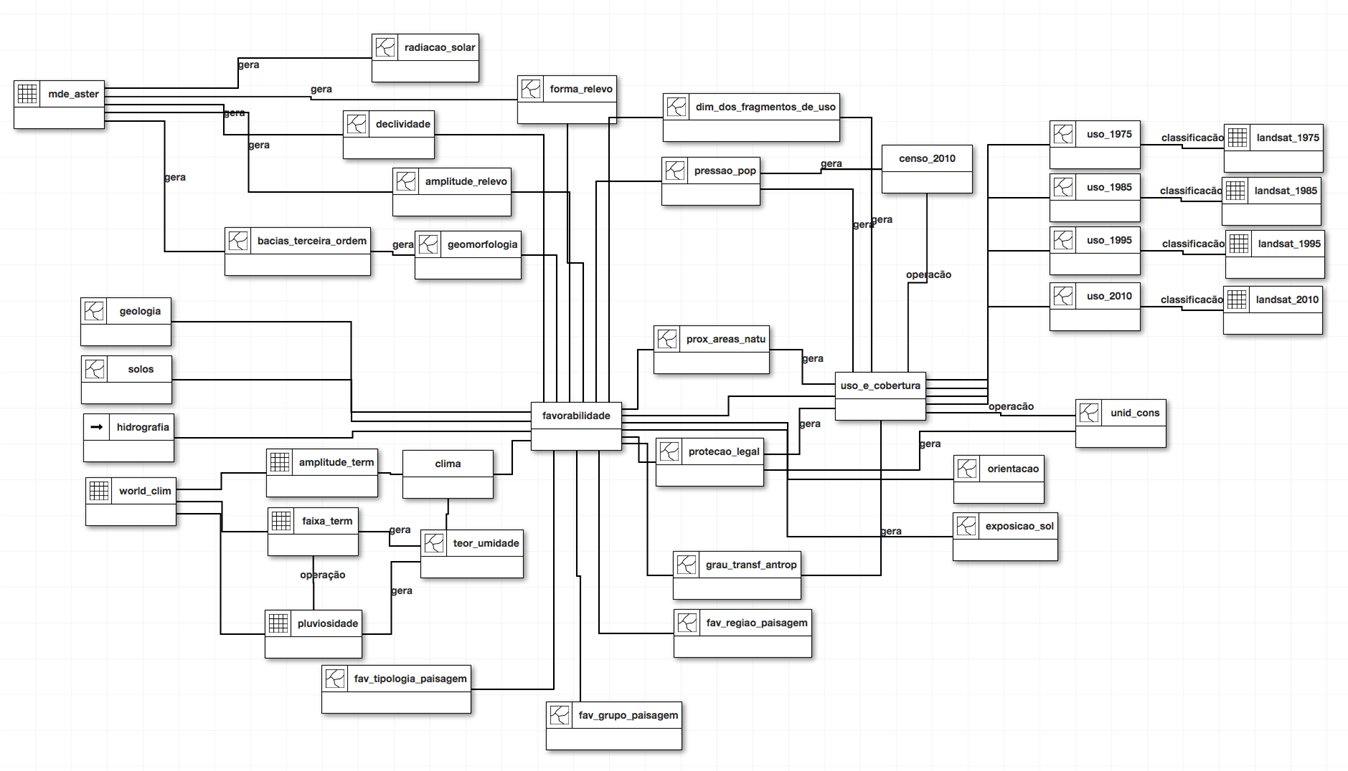
\includegraphics[width=1\linewidth]{data/modelo_OMT-G_final}
		\caption{Modelo OMT-G baseado no estudo realizado por Seabra (2012)\cite{SEABRA} na BHRSJ.}
		\label{fig:modeloomt-gfinal}
	\end{sidewaysfigure}

\newpage
\section{Implementação do modelo no PostGIS}

O banco de dados geográfico foi implementado utilizando o Sistema Gerenciador de Banco de Dados Objeto Relacional (SGBDOR) PostgreSQL versão 9.5 (64-bit) utilizando-se a extensão espacial PostGIS versão 2.2.2, assim como a interface gráfica pgAdmin versãoIII (Figura \ref{fig:pgadmin-gui}). 

	\begin{figure}
		\centering
		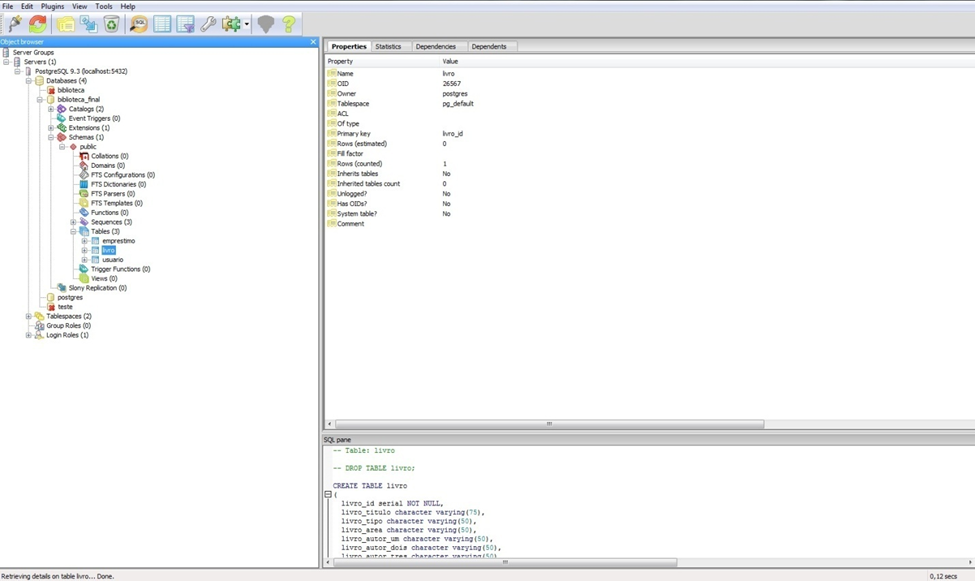
\includegraphics[width=1\linewidth]{data/pgAdmin-gui}
		\caption{Interface gráfica pgAdmin III utilizada para gerenciar o SGBDOR PostgreSQL assim como a extenção espacial PostGIS}
		\label{fig:pgadmin-gui}
	\end{figure}

A etapa de implementação do modelo OMT-G no banco PostGIS é relativamente rápida e simples. Através do pgAdmin podemos criar um novo banco de dados (Figura \ref{fig:newdbpgadmin}).

	\begin{figure}
		\centering
		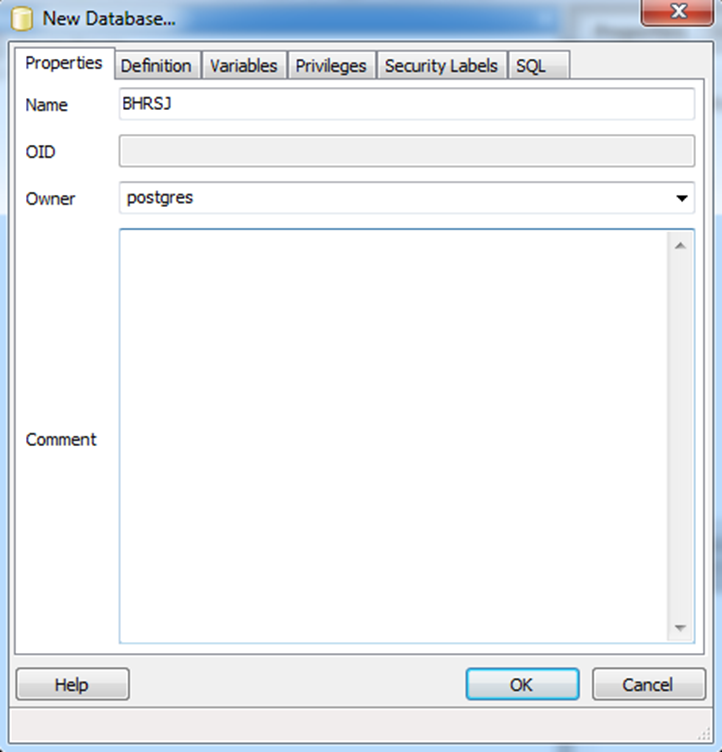
\includegraphics[width=0.6\linewidth]{data/newdb_pgadmin}
		\caption{Janela de criação de bancos no PostgreSQL 9.5 utilizando a interface pgAdmin III.}
		\label{fig:newdbpgadmin}
	\end{figure}
	
Após este processo, devemos dizer ao banco recém criado que gostaríamos de utilizar a extensão espacial PostGIS, ou seja, devemos dizer ao banco que queremos transformá-lo em um banco geográfico através de uma consulta SQL. A princípio, a ideia de adicionar a extensão espacial PostGIS através de uma consulta SQL pode parecer estranha, mas é o único método possível. Outras extensões com o \textit{pgRouting}, \textit{PostGIS Topology}, \textit{Point Cloud}, o módulo \textit{raster}, assim como outros, podem ser adicionados em um único comando:

	\begin{minipage}{\linewidth}
	\begin{lstlisting}
		CREATE DATABASE BHRSJ;
		\connect BHRSJ;
		-- Inicia a extensao PostGIS (ja inclui o modulo raster)
		CREATE EXTENSION postgis;
		-- Inicia a extensao Topology
		CREATE EXTENSION postgis_topology;
		-- Inicia a extensao PostGIS Advanced 3D 
		-- assim como outros algoritmos de geoprocessamento
		-- Inicia as extensoes relacionadas a geocoding
		CREATE EXTENSION postgis_sfcgal;
		CREATE EXTENSION fuzzystrmatch;
		CREATE EXTENSION address_standardizer;
		CREATE EXTENSION address_standardizer_data_us;
		CREATE EXTENSION postgis_tiger_geocoder;
		-- Inicia a extensao pgRouting para trabalhos que utilizam analise de rota
		CREATE EXTENSION pgrouting;
		-- Inicia a extensao pgr_fdw para adicionar outros tipos de dados externos
		CREATE EXTENSION ogr_fdw;
		
		-- Suporte para dados de LIDAR
		CREATE EXTENSION pointcloud;
		CREATE EXTENSION pointcloud_postgis;
	\end{lstlisting}
	\end{minipage}

No entanto, nem sempre é necessário adicionar todas as extensões em todos os projetos. Grande parte dos projetos, assim como este, utilizam apenas o módulo principal, iniciado através do comando "CREATE EXTENSION postgis;" (Figura \ref{fig:createextensionpostgis}). Após a execução deste comando, o PostgreSQL criará automaticamente uma tabela em seu banco nomeada "spatial ref sys" contendo o número de identificação de todos os 3911 códigos EPSG representando os sistemas de referência catalogados pela \textit{International Association of Oil and Gas Producers}. No Brasil, alguns códigos EPSG são mais utilizados do que outros, como o 4326 (WGS 84), o 4618 (SAD 69) e o 4674 (SIRGAS 2000)

	\begin{figure}
		\centering
		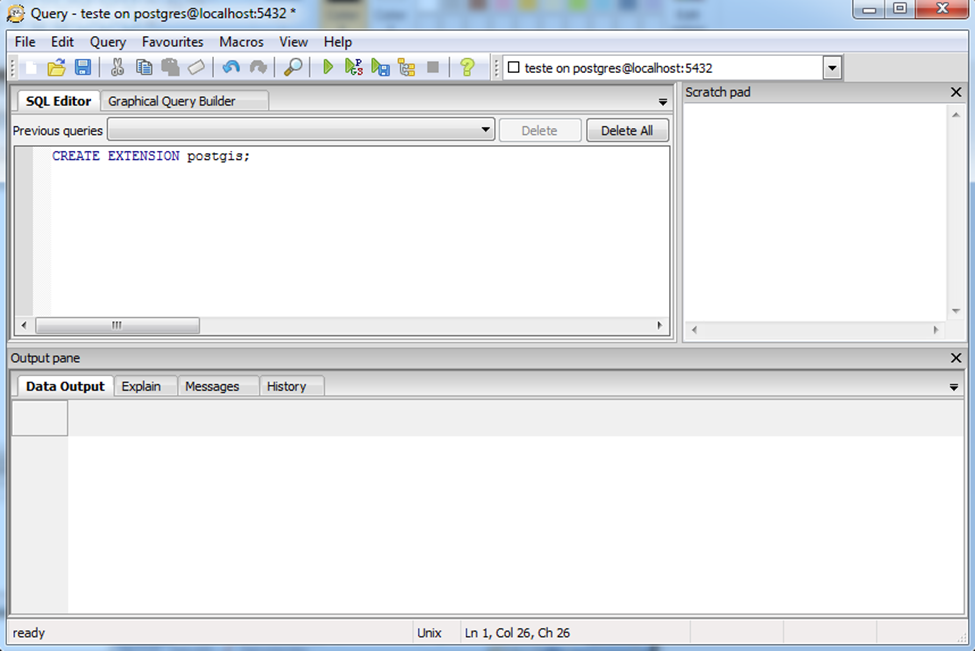
\includegraphics[width=1\linewidth]{data/create_extension_postgis}
		\caption{Através da consulta "\textbf{create extension postgis}" o banco recém-criado já poderá utilizar as funcionalidades espaciais.}
		\label{fig:createextensionpostgis}
	\end{figure}

Após a etapa de criação do banco e da inicialização da extensão PostGIS, inicia-se a etapa de importação de todos os dados definidos a serem inclusos pela nossa modelagem OMT-G. A importação de dados georreferenciados é diferente das importações de simples tabelas. Para esta etapa utilizamos um \textit{plugin} chamado PostGIS Shapefile and DBF Loader 2.1 (Figura \ref{fig:shapefileloader}). Nas últimas versões instaladas através do instalador oficial, o \textit{plugin} de importação de \textit{shapefiles} já vem incluso e instalado por padrão, sendo ainda mais fácil de importar dados em formato \textit{shapefile}. Para a importação de dados georreferenciados em outros formatos é necessário a utilização de outros \textit{plugins} como osm2pgsql que importa dados derivados do projeto OpenStreetMap para o PostGIS. Caso o plugin não esteja funcionando ou não o tenha instalado ainda é possível adicionar \textit{shapefiles} utilizando o Prompt de Comando e a ferramenta shp2pgsql e adicionando e executando o arquivo .sql criado na ferramenta de consultas SQL do pgAdmin:

	\begin{lstlisting}[float,floatplacement=H]
		shp2pgsql -s SRID shapefile.shp nome_da_tabela > shapefile.sql
	\end{lstlisting}

	\begin{figure}
		\centering
		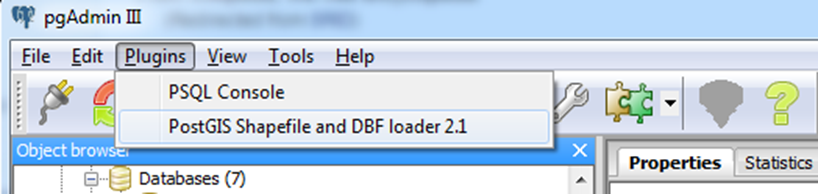
\includegraphics[width=1\linewidth]{data/shapefile_loader}
		\caption{Shapefile and DBF Loader 2.1.}
		\label{fig:shapefileloader}
	\end{figure}
	
Ao utilizar a interface gráfica do \textit{plugin} é importante que se configure o SRID (\textit{Spatial Reference System Identifier}) de cada \textit{shapefile} adicionado (Figura \ref{fig:shapefileloadergui}). É possível também adicionar múltiplos \textit{shapefiles} e/ou arquivos .dbf ao mesmo tempo. Além disso, é provável que seja necessário configurar a codificação do arquivo .dbf adicionado de OTF-8 para LATIN1 caso a tabela de atributos do \textit{shapefile} adicionada contenha caracteres típicos da linha portuguesa (Figura \ref{fig:importconfig}).

Outra funcionalidade da ferramenta de importação é a possibilidade de executar os algoritmos de indexação espacial como o GiST (\textit{Generalized Search Tree}) por padrão, já na etapa de importação e sem a necessidade de executar comandos SQL, como o demonstrado a seguir por exemplo:
	
	\begin{lstlisting}[float,floatplacement=H]
		CREATE INDEX nome_da_tabela_gix ON nome_da_tabela USING GIST (the_geom);
	\end{lstlisting}

	\begin{figure}
		\centering
		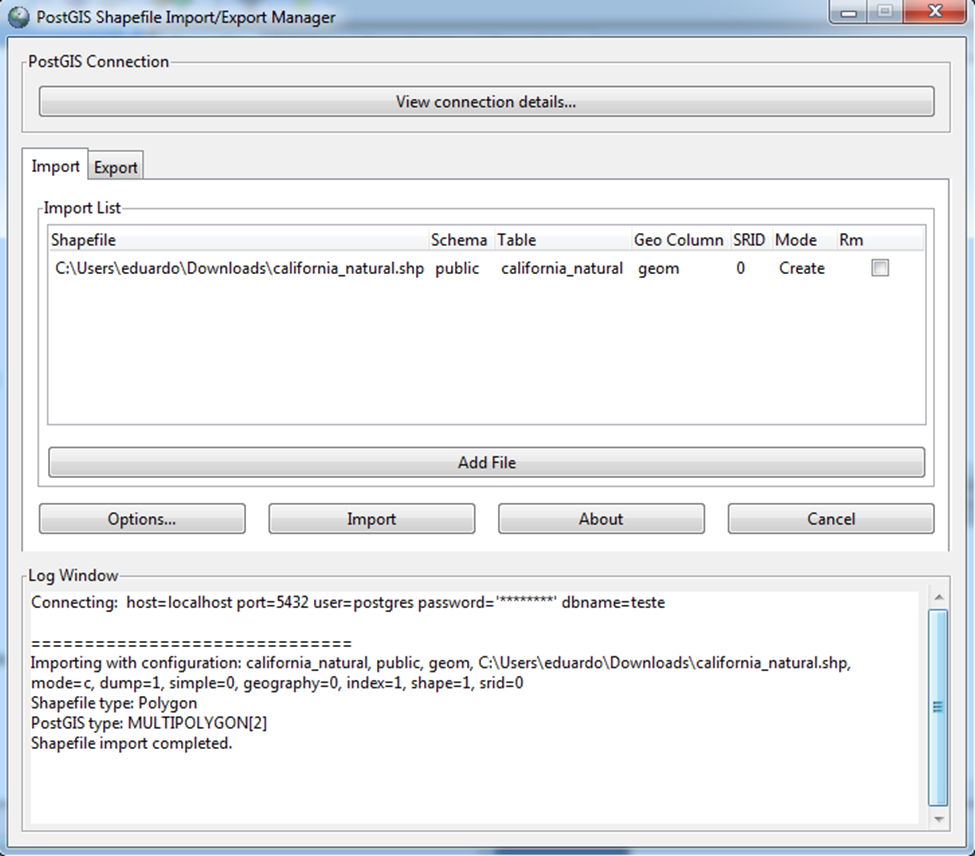
\includegraphics[width=1\linewidth]{data/shapefile_loader_gui}
		\caption{Interface gráfica do Shapefile and DBF Loader 2.1.}
		\label{fig:shapefileloadergui}
	\end{figure}
	
	\begin{figure}
		\centering
		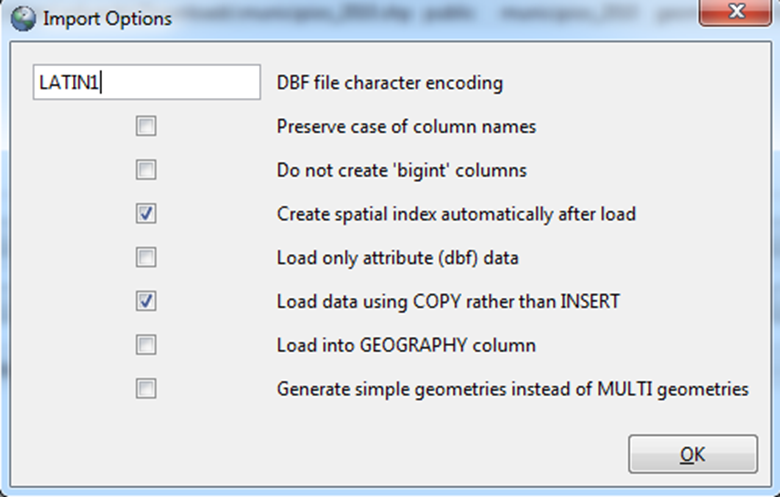
\includegraphics[width=1\linewidth]{data/import_config}
		\caption{Janela de configuração de importação. É interessante configurar o \textit{encoding} para LATIN1 para evitar caracteres estranhos e indesejados nos resultados das consultas.}
		\label{fig:importconfig}
	\end{figure}

	\section{Integração dos dados para análise}
	
	Com os dados já importados no PostGIS, é possível integrá-los com uma grande gama de aplicações tanto de forma offline quanto online. A partir daí muitas soluções de integração podem ser desenvolvidas. Uma bastante popular é representada na Figura \ref{fig:estruturaopensource} e utiliza a base de dados no PostGIS integrada ao Geoserver para a geração dos mapas consultados no PostGIS e visualizados em uma interface web como o OpenLayers. Uma abordagem mais específica e que demonstra todas as ferramentas e linguagens envolvidas no processo pode ser visto da Figura \ref{fig:estruturaopensource}. Outras já passam a utilizar tecnologias como Node.js com Express e Mapnik para criar servidores de mapas que processam a informação geográfica em "tempo real", sendo assim uma ótima alternativa para soluções em engenharia de tráfego e solucionamento de rotas, por exemplo.
	
	\begin{figure}
		\centering
		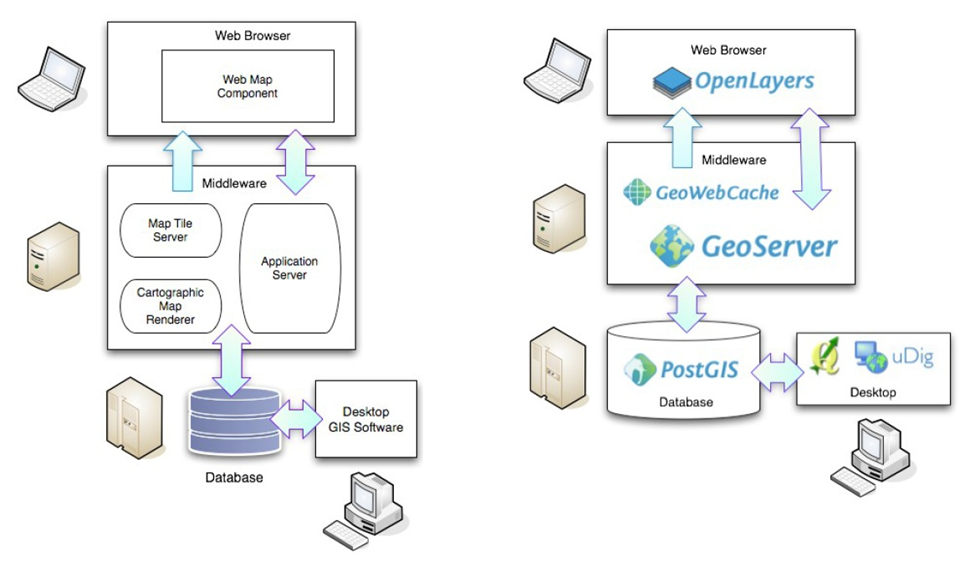
\includegraphics[width=1\linewidth]{data/estrutura_opensource}
		\caption{: Estrutura de código aberto que foi utilizada no trabalho e a representação da interface usuário/servidor. Autor: Carlos Cesar Gomes São Braz - IME(RJ)}
		\label{fig:estruturaopensource}
	\end{figure}

\newpage
	
No entanto, uma das principais e mais antigas ferramentas que possibilitam esta integração com o PostGIS é o QuantumGIS ou QGIS (Figura \ref{fig:diagrama}). O QGIS foi concebido inicialmente como uma ferramenta de conexão a bancos de dados PostgreSQL que utilizassem a extensão espacial PostGIS, mas que ao mesmo tempo tivesse como diferencial a funcionalidade de permitir a visualização do conteúdo geográfico para além das tabelas. O software amadureceu e hoje tem como bandeira ser o maior SIG gratuito e de código livre no mundo. No entanto, seu lado voltado aos bancos de dados desenvolveu somente até certo ponto. Em sua última versão estável 2.14 e mesmo em sua recém lançada versão de testes 2.16, o QGIS possui como padrão apenas a função de conexão e integração dos dados do PostGIS com o SIG. Alguns \textit{plugins} foram sendo desenvolvidos com o tempo por usuários que tentavam criar alternativas que buscassem simplificar ainda mais a utilização das funções exclusivas que o PostGIS possui. No entanto, nenhuma das alternativas apresentou, até o momento, uma interface que garanta um nível de abstração suficiente para que um usuário final que não saiba realizar consultas em SQL passe a utilizar estas funções espaciais.	

	\begin{figure}
		\centering
		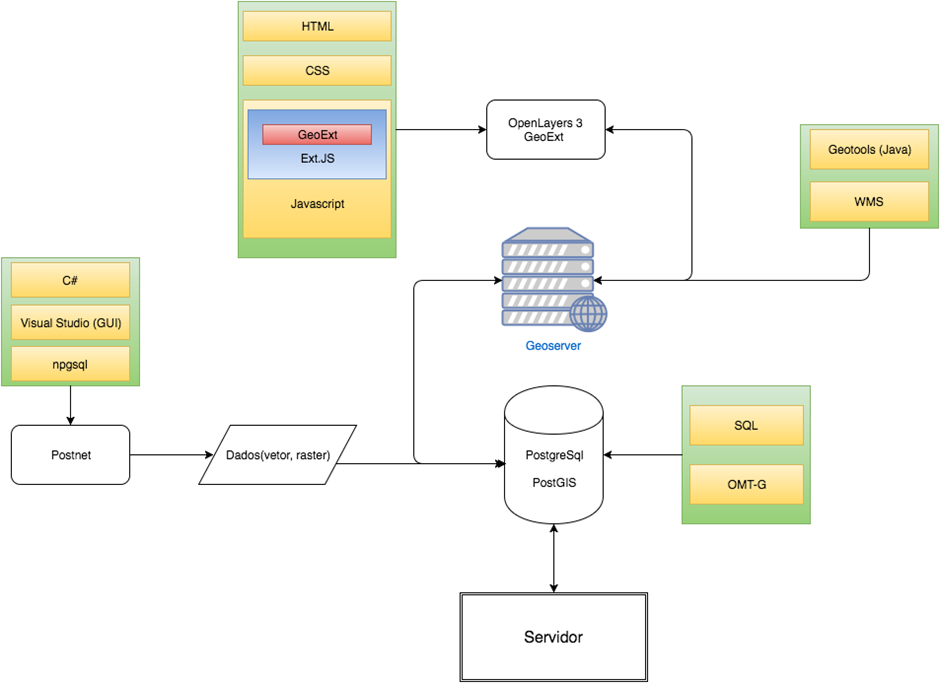
\includegraphics[width=1\linewidth]{data/diagrama}
		\caption{Diagrama com as ferramentas de análise, linguagens, recursos, suas conexões, camadas de abstração e tecnologias envolvidas.}
		\label{fig:diagrama}
	\end{figure}
	

	\begin{figure}
		\centering
		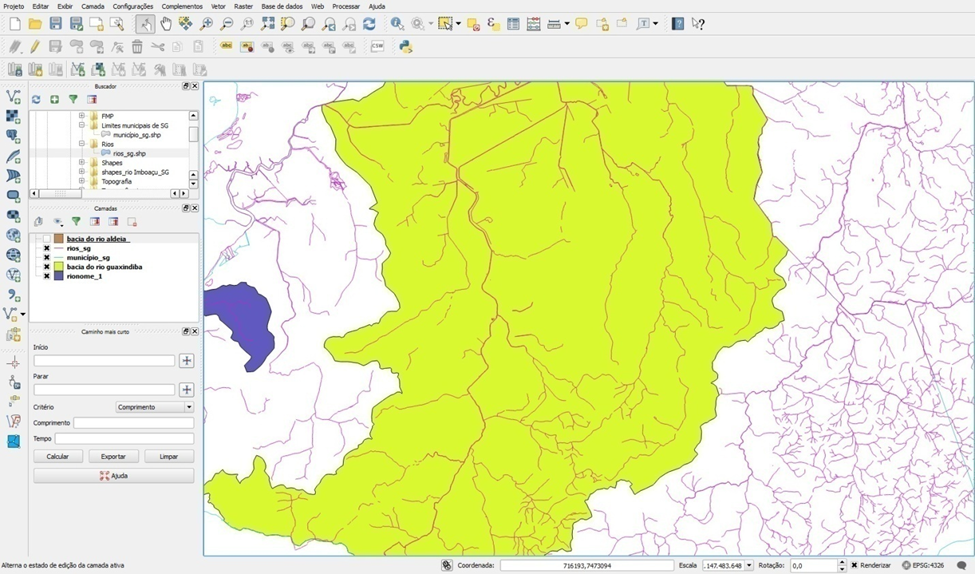
\includegraphics[width=1\linewidth]{data/qgis_gui}
		\caption{Interface gráfica do SIG QuantumGIS Desktop.}
		\label{fig:qgisgui}
	\end{figure}

A partir da proposta deste trabalho, pudemos notar nos capítulos anteriores que a utilização, por geógrafos, de banco de dados sejam eles geográficos ou não, na verdade já ocorre com certa frequência, mesmo que possibilitada por uma camada de abstração normalmente representada por uma funcionalidade do SIG como no caso do Geodatabase da ESRI. No entanto, por não existir um tipo de interface como o Geodatabase para plataformas livres, é importante considerar alternativas para que geógrafos e geocientistas de forma geral que utilizam ferramentas geoinformacionais livres também possam se beneficiar do uso de um SGBDOR, além de funcionalidades exclusivas sem que seja necessário aprender noções de programação e/ou SQL. 

Sendo assim, este trabalho buscou solucionar parte desse problema ao criar um software protótipo que possua uma interface gráfica que possibilite o usuário sem conhecimento técnico específico em programação, manipular informações geográficas mesmo que em grandes quantidades com o maior desempenho possível utilizando as funções de análise espacial do PostGIS.

Todo o desenvolvimento do software foi realizado utilizando a linguagem de programação C\# (C Sharp) através do \textit{framework} .NET e da IDE (\textit{Integrated Development Environment} -  Ambiente de Desenvolvimento Integrado) Microsoft Visual Studio 2015. C\# é uma linguagem interpretada multi-paradigma, fortemente tipada, e possui paradigmas de programação imperativa, funcional declarativa, genérica e principalmente orientada à objetos. É uma linguagem que foi desenvolvida pela Microsoft e foi apresentada oficialmente ao público em 2001 como parte do \textit{framework} .NET. por uma equipe montada e liderada por Anders Hejlsberg, criador do Delphi e do Turbo Pascal. Assim como Java, necessita ser compilada para \textit{bytecode} e interpretada por uma máquina virtual, neste caso, a \textit{Common Language Runtime} ou CLR. É uma linguagem que possui características muito próximas ao Java, o que por consequência faz com que grande parte das soluções desenvolvidas por ambas possuam características estruturais parecidas e possuam o mesmo "público alvo". A sintaxe utilizada pelo C\# se assemelha a vista em linguagens como C e C++, mesmo não possuindo relação direta com as mesmas. Além disso, linguagens como C e C++ possuem um processo de desenvolvimento muito mais complexo e são compiladas diretamente e especificamente para a arquitetura no qual o código foi compilado. 

Outra proposta do C\# (assim como do Java), é o de gerar códigos mais seguros e com menos chance de erros relacionados ao uso da memória. Em linguagens como C/C++, a utilização de ponteiros e a possibilidade de manipulação da memória ram através da \textit{Stack} e da \textit{Heap}, são essenciais para o desenvolvimento de softwares que buscam alto desempenho, mas necessitam que o programador saiba exatamente como e onde cada segmento de memória está sendo alocado e desalocado. Caso contrário, o programa tende a apresentar um número muito maior de \textit{bugs} e um uso excessivo de memória. Além disso, em projetos maiores e com número maior de linhas de código, a manutenção tende a ser muito mais complexa, assim como a identificação de erros relacionado ao mau uso de recursos. Tanto o C\# quanto o Java, são linguagens em que a utilização de recursos é em grande parte trabalho da máquina virtual e é consequentemente realizada de forma automática, sem que o desenvolvedor tenha que se preocupar. No entanto, há perda de desempenho.

Java foi por muito tempo a linguagem para aplicações \textit{desktop} que possuía um lado web que dominou a área do desenvolvimento geotecnológico. Ferramentas como o GeoTools, GeoServer, JTS Topology Suite, Gisgraphy, e o World Wind Java SDK desenvolvido pela NASA, são bons exemplos de como a comunidade de desenvolvedores SIG tinham uma preferência clara em relação à linguagem Java. O provável motivo para tal preferência eram as características multi-plataforma de uma linguagem livre como o Java e seu consequente crescimento em todo o mercado de TI. O C\#, por ter sido desenvolvido pela Microsoft tinha como limitação a dependência do sistema Windows para rodar suas aplicações. No entanto, com o tempo, muitas soluções multi-plataformas foram surgindo como o Mono e posteriormente o Xamarin até a liberação total das bibliotecas padrões oficialmente pela Microsoft. Sendo assim, hoje em dia, C\# é uma linguagem de programação livre e também multi-plataforma (Windows, Linux, OSX, Android, iOS, Windows Phone, etc). 

Na área geoespacial, algumas ferramentas importantes foram desenvolvidas nos últimos 15 anos utilizando C\# como o SharpMap.NET, o NTS Topology Suite (versão em C\# do JTS escrito em Java), o GeoLib, o Nutiteq Maps SDK (para plataformas mobile), e mais recentemente o DotSpatial, ferramenta base deste trabalho.

O DotSpatial é uma biblioteca escrita originalmente para o \textit{framework} .NET 4 utilizando a linguagem C\# como uma solução para incorporar funções SIG para outras aplicações. Este projeto utilizou o DotSpatial para adicionar funções básicas de manipulação de dados georreferenciados em um ambiente simples. Além disso, o sistema possui uma segunda interface para a manipulação de funções espaciais do PostGIS. 

Toda a funcionalidade de conexão com o banco de dados PostgreSQL/PostGIS foi realizada utilizando-se da biblioteca Npgsql (NPGSQL, 2016) buscando utilizar as funcionalidades proporcionadas pelo paradigma da programação orientada a objetos.

Sendo assim, através da possibilidade de utilização das citadas ferramentas iniciou-se o processo de desenvolvimento de um Sistema de Informações Geográficas protótipo denominado espaçoGIS (Figura \ref{fig:espacogislogo}).

	\begin{figure}
		\centering
		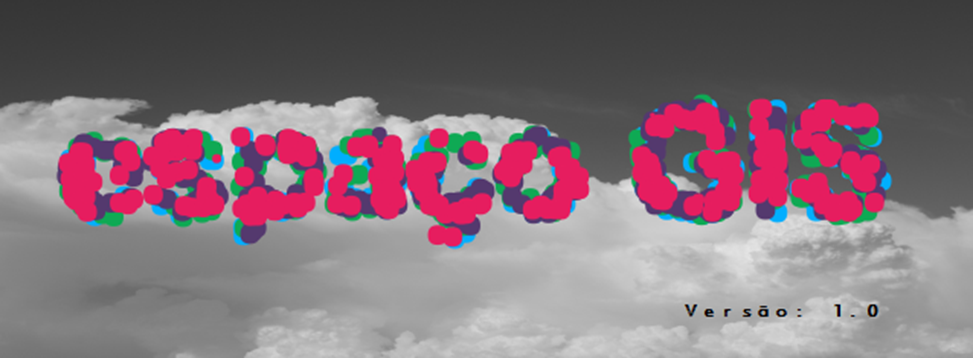
\includegraphics[width=1\linewidth]{data/espacoGIS_logo}
		\caption{Logo do Sistema de Informação Geográfico espaçoGIS.}
		\label{fig:espacogislogo}
	\end{figure}

O protótipo utiliza uma interface de documentos múltiplos (MDI - \textit{Multiple Document Interface}) para gerenciar as janelas, dando a possibilidade de gerenciamento dos diversos módulos pertencentes ao SIG espaçoGIS (Figura \ref{fig:espacogisgui}), como o módulo SIG e o módulo de funcionalidades e gerenciamento de bancos de dados no PostGIS denominado PostNet (Figura \ref{fig:postnetgui}). Na Figura \ref{fig:mdigui} apresenta a vantagem do uso de uma interface do tipo MDI.

	\begin{figure}
		\centering
		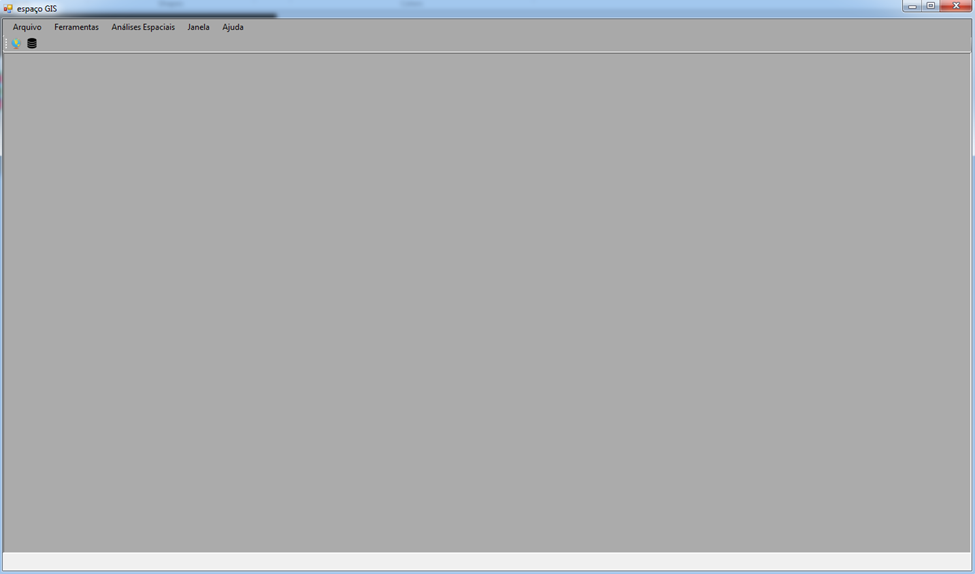
\includegraphics[width=0.8\linewidth]{data/espacoGIS_gui}
		\caption{Apresentação inicial da interface do sistema espaçoGIS.}
		\label{fig:espacogisgui}
	\end{figure}
	
	\begin{figure}
		\centering
		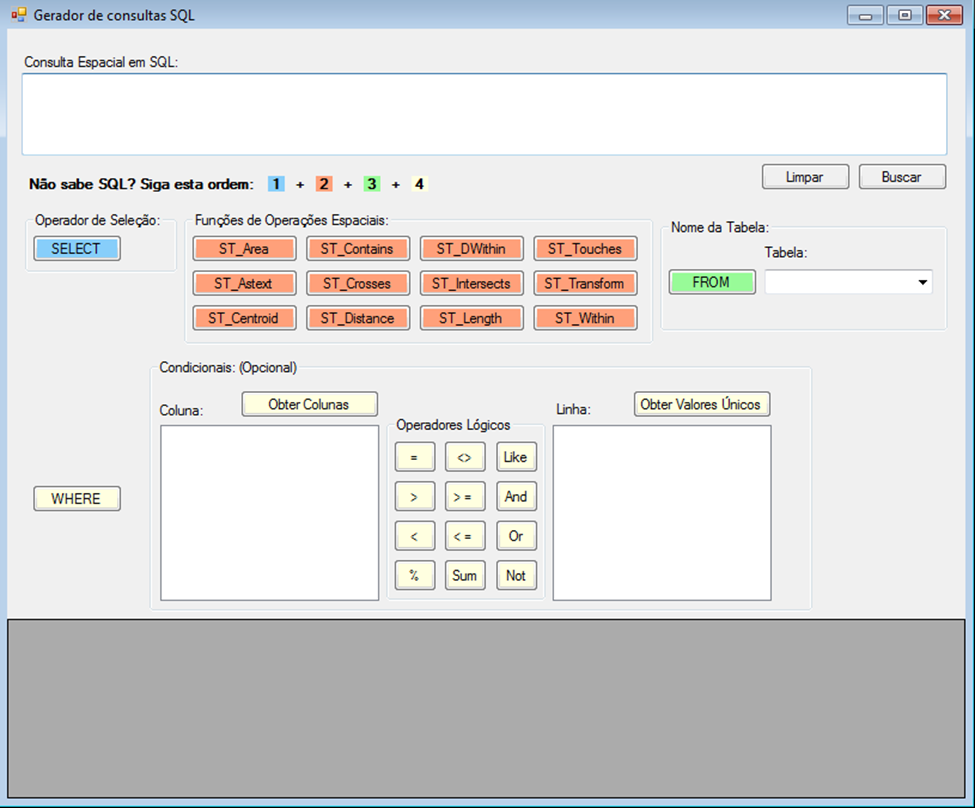
\includegraphics[width=1\linewidth]{data/postnet_gui}
		\caption{Módulo PostNET ou "Gerenciador de Consultas SQL".}
		\label{fig:postnetgui}
	\end{figure}

	\begin{figure}
		\centering
		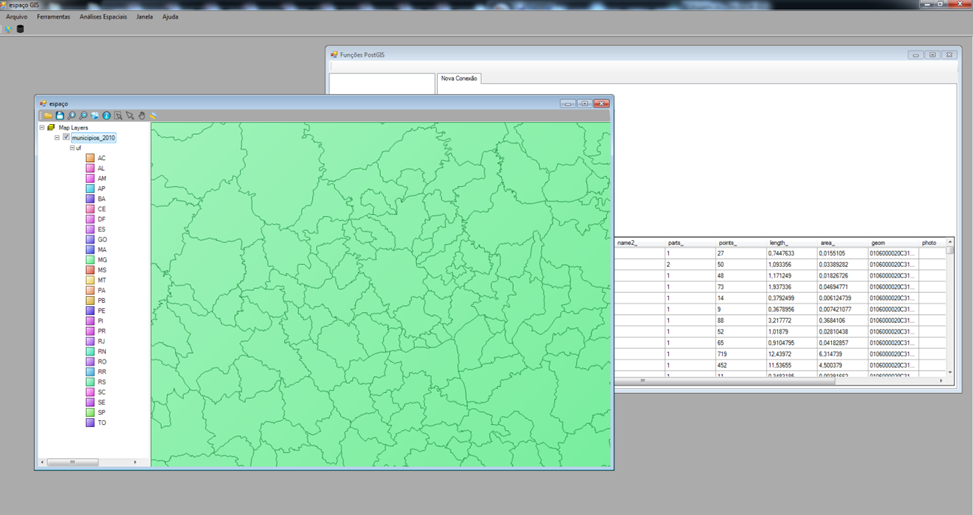
\includegraphics[width=1\linewidth]{data/mdi_gui}
		\caption{A escolha pelo uso de um MDI se deu em função da implementação de diversos módulos em um mesmo sistema.}
		\label{fig:mdigui}
	\end{figure}

A implementação do módulo SIG se deu primeiramente desenvolvendo as funcionalidades mais básicas utilizando a biblioteca DotSpatial. Funções como "Adicionar Camada", "Zoom In", "Zoom Out", "Zoom to Extent", "Limpar Camada", "Informações", "Selecionar", "Pan" e "Salvar Camada" foram implementadas primeiramente como mostrado no Anexo.

Em seguida, o módulo de funções ligadas à aba de legenda foi desenvolvida assim como o módulo de visualização dos mapas, representados respectivamente na Figura \ref{fig:siggui}.

A interface ainda possui a janela de conexão ao PostGIS (Figura \ref{fig:postgisconfig}) e ao módulo PostNET. A GUI (\textit{Guafical User Interface}) desenvolvida para as funções do módulo PostNet possuem um padrão específico, buscando se assemelhar propositalmente à interface do módulo "Selecionar por Atributos" desenvolvida para o SIG ArcMap. Esta escolha se deu devido a grande popularidade do software e por considerar que grande parte da comunidade envolvida com a utilização de SIG provavelmente já teve algum contato com a ferramenta da ESRI, facilitando o acesso de novos usuários.

	\begin{figure}
		\centering
		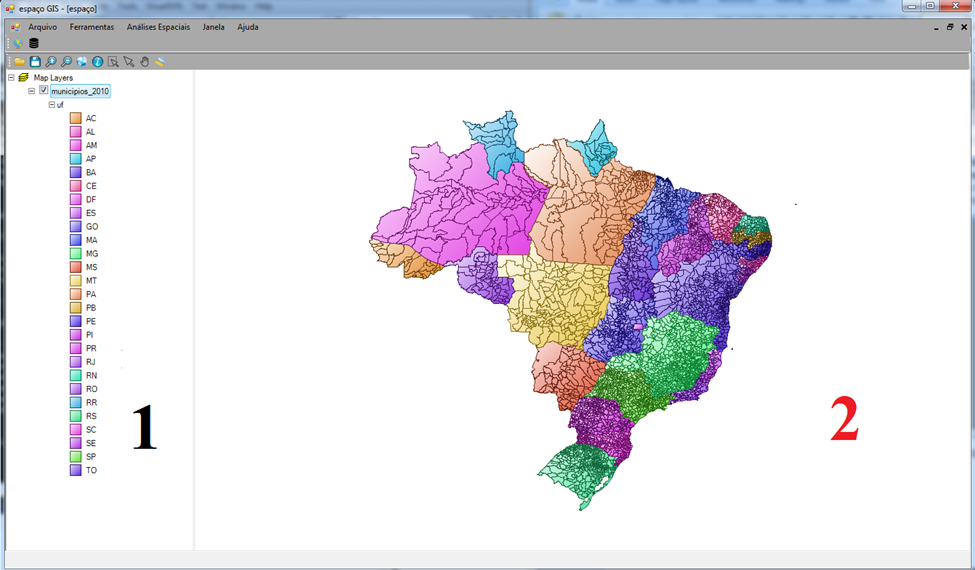
\includegraphics[width=1\linewidth]{data/sig_gui}
		\caption{A interface gráfica do módulo SIG é dividido basicamente entre duas áreas de visualização. A área de legenda, organização dos \textit{layers} e funcionalidades de visualização e exportação representada pelo número 1 e a área de visualização de mapas representada pelo número 2.}
		\label{fig:siggui}
	\end{figure}
	
	\begin{figure}
		\centering
		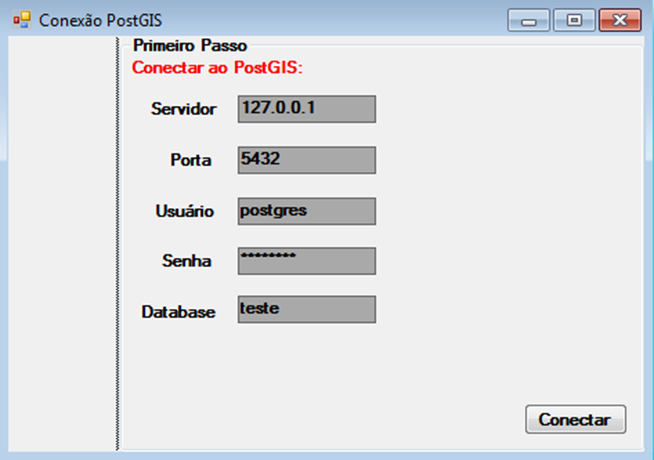
\includegraphics[width=0.7\linewidth]{data/postgis_config}
		\caption{Janela de configuração de conexão com o banco PostGIS.}
		\label{fig:postgisconfig}
	\end{figure}
	
O propósito pela criação de uma ferramenta com uma interface como o PostNET é a de facilitar o aprendizado da linguagem SQL padrão, assim como principalmente da sintaxe utilizada pelo módulo PostGIS.

\chapter{Considerações Finais}
A busca por uma Geografia mais conjuntiva, integrada e transdisciplinar é o que motiva a busca por novas metodologias de análise e futuras discussões epistemológicas de acordo com o constante avanço tecnológico. A percepção e inclusão da noção de espaço pela ciência atual como um aditivo ao conceito de tempo, já tradicional em muitos estudos, explica a necessidade por trabalhos que provoquem esta maior integração na Geografia. A preocupação pela inclusão da espacialidade ao explicar processos com mudanças ao longo do tempo gerou como resposta uma busca pelo desenvolvimento de ferramentas que suportem, de fato, estas análises. 

Além disso, o rápido desenvolvimento de tecnologias de armazenamento e processamento de dados digitais, assim como sua popularização e distribuição em massa geraram como consequência um aumento significativo na acumulação de informações espacializadas. No entanto, apesar de tal desenvolvimento, a Geografia parece, de forma geral, enfrentar limitações quando o assunto é a integração de métodos computacionais modernos ao processo de análise espacial. Limitações como esta tem origem epistemológica e são consequência de uma lógica do fazer científico que esbarra em uma histórica lógica Kuhniana de quebra de paradigmas. Entendendo o desenvolvimento do pensamento não só geográfico, como científico, principalmente durante o último século, nos revela que a busca por uma Geografia menos dicotômica pode ser a chave para uma ciência geográfica mais integrada e transdisciplinar.

A aplicação de métodos computacionais na Geografia possui uma longa história, e pelo o que o desenvolvimento de tecnologias recentes vem mostrando, esta relação tende a aumentar como nunca. Cabe, portanto a Geografia buscar entender como a aplicação de novas tecnologias pode sim influenciar na integração de análises geográficas quantitativas e qualitativas. 

Este trabalho buscou contribuir para a discussão mostrando que esta relação não necessariamente precisa ser feita através de grandes especialistas técnicos. Além disso, teve como objetivo a criação de uma ferramenta que possa servir como base para que pesquisadores ou qualquer maior interessado aprenda e utilize todo o potencial que os bancos de dados geográficos e suas análises espaciais disponibilizam.

O fazer científico atual baseado na acumulação de grandes bases de dados espaciais possui muitos perigos em sua utilização, principalmente quando tratado como finalidade. A Geografia, especialmente a brasileira, possui discussões conceituais aprofundadas que podem ajudar este novo paradigma a encontrar um caminho um pouco mais crítico. No entanto, é necessário que se olhe para novas tecnologias sem o medo burro do preconceito e entendendo que o fazer científico, sendo quantitativo ou não, deve ser feito com consciência. 

Além disso, compreender as funcionalidades existentes nas implementações dos SIG existentes nos dá a possibilidade de entender o processo de produção do conhecimento geotecnológico compatível com as limitações impostas pela tecnologia desenvolvida. Ou seja, se o software de SIG padrão determina a pesquisa e a prática do SIG, a utilização de bancos de dados geográficos que permitam uma análise geográfica mais completa e funcional, podem por consequência influenciar na produção de estudos geográficos mais complexos.

A criação de novas técnicas e ferramentas é constante e foi percebida na própria realização deste trabalho devido as constantes atualizações na bibliografia. Buscou-se citar a maior parte das principais ferramentas de análise espacial ligadas a utilização de bancos de dados geográficos, no entanto, não há tempo para um estudo mais aprofundado para cada tecnologia. Priorizou-se então a busca em entender a diversidade de ferramentas e métodos.

De forma geral, a Geografia brasileira atual buscar formar o novo geógrafo centrado no entendimento de seus conceitos fundamentais e na realização de análises geográficas de forma a considerar particularidades, ações e objetos em múltiplas escalas. A aplicação de conceitos como o de holística e complexidade surgem neste contexto como uma sensação de otimismo aos que não conseguem entender duas geografias. De acordo com o aprimoramento tecnológico, pouco a pouco, conceitos fundamentais da Geografia talvez poderão ser aplicados a novas soluções. Cabe a Geografia então servir como norteadora para um desenvolvimento geotecnológico, de fato, mais integrado.